\documentclass[11pt]{article}
\usepackage{../../EllioStyle}
\usepackage{fancyvrb}
\usepackage{listings}
\usepackage{multicol}
\usepackage{forest}

\definecolor{codegreen}{rgb}{0,0.6,0}
\definecolor{codegray}{rgb}{0.5,0.5,0.5}
\definecolor{codepurple}{rgb}{0.58,0,0.82}
\definecolor{backcolour}{rgb}{0.95,0.95,0.92}

\lstdefinestyle{mystyle}{
%    backgroundcolor=\color{backcolour},   
    commentstyle=\color{codegreen},
    keywordstyle=\color{magenta},
    numberstyle=\tiny\color{codegray},
    stringstyle=\color{codepurple},
    basicstyle=\ttfamily\footnotesize,
    breakatwhitespace=false,         
    breaklines=true,                 
    captionpos=b,                    
    keepspaces=true,                 
    numbers=left,                    
    numbersep=5pt,                  
    showspaces=false,                
    showstringspaces=false,
    showtabs=false,                  
    tabsize=2
}

\title{Comparison of Algorithms for Multiple Sequence Alignment}
\author{Elliott Pryor}
\date{16 December 2021}

\rhead{Comparison of Algorithms for Multiple Sequence Alignment}

\begin{document}
\maketitle

\section{Introduction}
\label{sec:intro}

Multiple Sequence Alignment (MSA) seeks to find the optimal global alignment of a set of $k$ input strings.
This is a generalization of the global alignment problem to three or more strings.
The goal is to align strings $1, \dots, k$ in order to minimize a scoring function (see Equation \ref{eq:SP}). 
Finding the optimal MSA alignment has been shown to be NP-Complete \cite{wang1994complexity}.
So different heuristic methods are applied in order to approximate the MSA alignment.

In this work, we examine different MSA algorithms, Center-Star and ClustalW. 
We implement them in python and compare their running time as well as the quality of alignment produced.

\subsection{Global Alignment}
The global alignment problem seeks to find the optimal alignment of two strings, 
$S, T$ that minimizes some similarity function.
An alignment is constructed by inserting gaps at different locations into the strings. 
The length of the two aligned strings must be the same.
A common similarity function that is used in this work is given in Equation \ref{eq:edit_dist}.

\begin{equation}
    S = \sum_{i = 1}^n \delta(S[i], T[i]), \quad \delta(S[i], T[i]) = \begin{cases}
        0 & \text{if } S[i] = T[i] \\
        1 & \text{otherwise}
    \end{cases}
    \label{eq:edit_dist}
\end{equation}

We can see that if we have the same strings ($S = T$) the score is $0$ from Equation \ref{eq:edit_dist}.
The optimal alignment is the alignment of strings $S, T$ that minimizes the similarity score.  
For example consider the strings: $ACAATCC$ and $AGCATGC$. They have an optimal alignment with score of 3:

\begin{Verbatim}[commandchars=\\\{\}]
    A\textcolor{red}{_}CA\textcolor{red}{A}T\textcolor{red}{C}C
    A\textcolor{red}{G}CA\textcolor{red}{_}T\textcolor{red}{G}C
\end{Verbatim}

The global alignment problem is known to be solvable in $O(n^2)$ time where $n$ is the length of the longest input string
using the Needleman-Wunsch algorithm \cite{needleman1970general}.
The Needleman-Wunsch algorithm is a dynamic programming algorithm.
We construct an initial matrix $V = m \times n$, $V[0,0] = 0$, $V[j, 0] = j$, $V[0, i] = i$.
We assume that $S[0] = T[0] = \_$, then we can compute the optimal score by filling matrix V out using Equatin \ref{eq:needleman}.
The optimal score is $V[m, n]$. 
The optimal string alignment can be determined by backtracing along the optimal $b_1, b_2$ at each step.
\begin{equation}
    V[i,j] = \min_{(b_1, b_2) \in \{ (0, 1)\}^ 2 \setminus \{ (0,0)\})} 
    V[i-b_1, j-b_2] + \delta(S[i \cdot b_1], T[j \cdot b_2])
    \label{eq:needleman}
\end{equation}

\section{Methods}

\subsection{Optimal Dynamic Program}

This is an extension to the Needleman-Wunsch algorithm that extends to find the optimal solution to the MSA problem.
We already know that this problem is NP-Complete, so the algorithm runs in exponential time with respect to $k$ (the number of strings).
As a matter of fact the running time is $O(n^k 2^k k^2)$ and it uses $O(n^k)$ space.
This is not ideal, but it was expected. 
We first define the sum of pairs distance that is used to score MSA's. 
The formula to align a set of characters is given in Equation \ref{eq:SP}
 (we note this function is a parallel of $\delta$ in the global alignment problem).
If we want to compute the score of an MSA, then $SOP(S_1, \dots, S_k) = \sum_{i = 1} ^n SP(S_1[i], \dots , S_k[i])$

\begin{equation}
    SP(a_1, \dots, a_k) = \sum_{1 \leq i < j \leq k} \delta(a_i, a_j)
    \label{eq:SP}
\end{equation}

The algorithm is a very simple extension to the Needleman-Wunsch algorithm. 
Instead of creating $V$ to be a two dimensional matrix, we create $V$ to be a $k$-dimensional tensor. 
The tensor is filled out using Equation \ref{eq:opt}

\begin{equation}
    V[i_1, \dots, i_k] = \min_{(b_1, \dots, b_k) \in \{ (0, 1)\}^ k \setminus \{ (0, \dots, 0)\})}
    V[i_1-b_1, \dots, i_k-b_k] + SP(S_1[i_1 \cdot b_1], \dots, S_k[i_k \cdot b_k])
    \label{eq:opt}
\end{equation}

We impose the restriction that if $i_j = 0$ then $b_j = 0$ this prevents us from indexing outside of the tensor.
Similarly to Needleman-Wunsch, 
the optimal alignment can be recovered by backtracking along the optimal $\vec{b}$ at each index.


\subsection{Center Star}
Center Star is a $2$-approximation algorithm for MSA. 
This means that $SOP(\text{center star}) \leq 2 * SOP(\text{optimal})$.
This performance guarantee is very nice and can be very useful in applications
where the score cannot be too far away from optimal.
The running time is $O(k^2 n^2)$.

\begin{algorithm}[H]
    \caption{Center Star Algorithm}
    \label{alg:center_star}
    \begin{algorithmic}[1]
    \Function{Center-Star}{$S_1, \dots, S_k$}
        \State K = kxk matrix, $K[i,j] = $edit distance between $S_i, S_j$
        \State Compute distance to other strings $D_i = \sum_{j=1}^k K[i,j]$
        \State take center string $S_c$, where $c = argmin_{i} D_i$
        \State Compute alignments with $S_c$
        \State Merge alignments together (need to add spaces into $S_c$)
    \EndFunction
    \end{algorithmic}
\end{algorithm}

In line 2, we compute the pairwise distances between all strings, 
the edit distance is computed using the Needleman-Wunsch algorithm.
Then in line 4 we find the center string $S_c$ that minimizes the sum of distances to all other strings.
We then create the optimal alignment by sequentially merging pairwise alignments.
We align $S_i, S_c$ using Needleman-Wunsch. 
Then if there is a blank introduced into $S_c$, 
we insert a blank at this location in all previously aligned sequences $S_{i - j}$ for $j > 0$.
We note that aligning the next string in the sequence $S_i$ with $S_c$ uses the current version of $S_c$ 
(that has blanks from previously aligned strings).

\subsection{ClustalW}
ClustalW is a popular heuristic for computing MSA. 
ClutalW was proposed by Thomson et. al. in 1994 \cite{thompson1994clustal}
It does not have a proven performance guarantee. But is very commonly used to compute MSA in practice.
It runs in $O(k^2 n^2 + k^3)$ time. 
I was not able to find any psudocode describing the algorithm,
so one of the main contributions of this work is to provide clear psudocode.
The main steps of the ClustalW algorithm are:

\begin{enumerate}
    \item Calculate all possible pairwise alignments, record the score for each pair.
    \item Calculate a guide tree based on the pairwise distances via Neighbor Joining.
    \item Find the two most closely related sequences
    \item Align the sequences by progressive methods (profile-profile alignment)
    
    \begin{enumerate}
        \item Calculate a consensus of this alignment
        \item Replace the two sequences with the consensus
        \item Find two next most closely related sequences
    \end{enumerate}

    \item report the MSA
\end{enumerate}

Step one is easy, it is the same as line 2 in Algorithm \ref{alg:center_star}. 
There is also no very useful algorithm for neighbor joining algorithm.
The most clear implementation is on \href{https://en.wikipedia.org/wiki/Neighbor_joining}{Wikipedia}.

\begin{algorithm}[H]
    \caption{Neighbor Joining Algorithm}
    \label{alg:nj}
    \begin{algorithmic}[1]
    \Function{Neighbor-Join}{distance matrix $D$}
        \State Initialize $T$ star graph with one leaf for each taxa (string)
        \While{$D > 2 \times 2$ (D has more than 2 nodes)}
            
            \State $Q[i,j] = (n-2) D[i, j] - \sum_{k=1}^n D[i, k] - \sum_{k=1}^n D[j, k]$
            \Comment \textit{Compute Q matrix}
            \State find $i, j$ with $i \neq j$ such that $Q[i,j]$ is minimized
            \State Connect $i, j$ into new node $u$ in $T$
            
            \State $\delta(i, u) = \frac{1}{2} D[i, j] + \frac{1}{2(n-2)} \left[\sum_{k=1}^n D[i,k] - \sum_{k=1}^n D[j,k] \right]$
            \Comment \textit{Compute distance from i,j to u}
            \State $\delta(j, u) = D[i, j] - \delta(i, u)$
            
            \State $D[u, k] = \frac{1}{2} \left[ d(i, k) + d(j, k) - d(i, j) \right]$
            \Comment \textit{Compute distances from all other nodes to u}
            \State Replace $i, j$ with node $u$ and using the distances computed in previous step
        \EndWhile
        \State \textbf{return} $T$
    \EndFunction
    \end{algorithmic}
\end{algorithm}

Now we have a guide tree, so we need to merge the sequences along it.
But when we are merging two nodes, if they are interior nodes then there are multiple sequences to align!
How do we do this?
We need a profile profile alignment score to align alignments $A_1, A_2$:
$$PSP(A_i[i], A_2[j]) = \sum_{x, y \in \Sigma} g_i(x), g_j(y \delta(x,y))$$
Where $\Sigma$ is the alphabet, $g_i(x)$ is the number of time $x$ occurs in column $i$ of $A_1$, 
and $g_j(y)$ is the number of time $y$ occurs in column $j$ of $A_2$.
We then can merge alignments using Needleman-Wunsch with the scoring function $PSP$.
In other words: $V[i,j] = \max \begin{cases}
    V[i-1, j-1] + PSP(A_1[i], A_2[j]) \\
    V[i-1, j] + PSP(A_1[i], \_) \\
    V[i, j-1] + PSP(\_, A_2[j])
\end{cases}$ 
Thus the progressive alignment algorithm is:

\begin{algorithm}[H]
    \caption{Progressive Alignment}
    \label{alg:nj}
    \begin{algorithmic}[1]
    \Function{Progressive-Align}{guide tree $T$ with leaves labeled $S_1, \dots , S_k$}
        \Repeat
        \State Choose two adjacent leaf nodes $u, v$ with parent $p$
        \State Compute profile-profile alignment using Needleman-Wunsch with $PSP$
        \State Label node $p$ with this alignment $A_3$
        \State remove $u, v$ from $T$
        \Until{only one node in $T$}
        \State \textbf{return} alignment label on last node remaining
    \EndFunction
    \end{algorithmic}
\end{algorithm}

Now we finally have all the pieces in order to give psudocode for the full ClustalW algorithm

\begin{algorithm}[H]
    \caption{ClustalW}
    \label{alg:nj}
    \begin{algorithmic}[1]
    \Function{ClustalW}{$S_1, \dots, S_k$}
        \State D = kxk matrix, $D[i,j] = $edit distance between $S_i, S_j$
        \State $T$ = Neighbor-Join(D)
        \State label leaf nodes of $T$ with $S_1, \dots, S_k$
        \State alignment = Progressive-Align($T$)
        \State \textbf{return} alignment
    \EndFunction
    \end{algorithmic}
\end{algorithm}

\section{Experiments}
\subsection{Experimental Setup}
The algorithms described above were implemented in python.
Their implementation can be found open sourced on 
\href{https://github.com/ElliottP-13/ComputationalBiology/tree/main/Project}{Github/ElliottP-13/ComputationalBiology}.
We cap the running time for the exact algorithm at 900 seconds. 
We do not kill the program after it exceeds 900 seconds, 
but we stop attempting to compute the optimal alignment.

We ran experiments using different number of strings all of length 50. 
We compare the running time for each algorithm to compute an MSA, as well as the $SOP$ score of the alignment
We generate three different topologies for $k$ random strings.

\begin{enumerate}
    \item Random - Generate $k$ purely random strings
    \item Center - Generate one center sequence, then $k-1$ strings with between 5 and 16 mutated characters.
    \item Tree - Generate root string. Generate 2 children with between 5 and 16 mutated characters. 
    Repeat until we have $k$ leaf nodes.
    We note that this simulates a binary phylogeny.
\end{enumerate}

\subsection{Results}

Results from experiments are shown in Figure \ref{fig:all_results}.
Comparisons of MSA scores are in Figure \ref{fig:centerScore} - \ref{fig:treeScore},
and comparisons of running time are in Figure \ref{fig:centerTime} - \ref{fig:treeTime}.
The exact algorithm was only able to compute MSA for 3 and 4 strings.
Computing MSA for 4 strings took over 20 minutes!
On the center string topology, center star was optimal for the 3 strings, and 1 away from optimal for 4.
This is expected given the nature of the topology. It is worth noting ClustalW also got optimal for 3 strings on center topology.

\begin{figure}
    \centering

    \begin{subfigure}[b]{0.49 \textwidth}
        \centering
        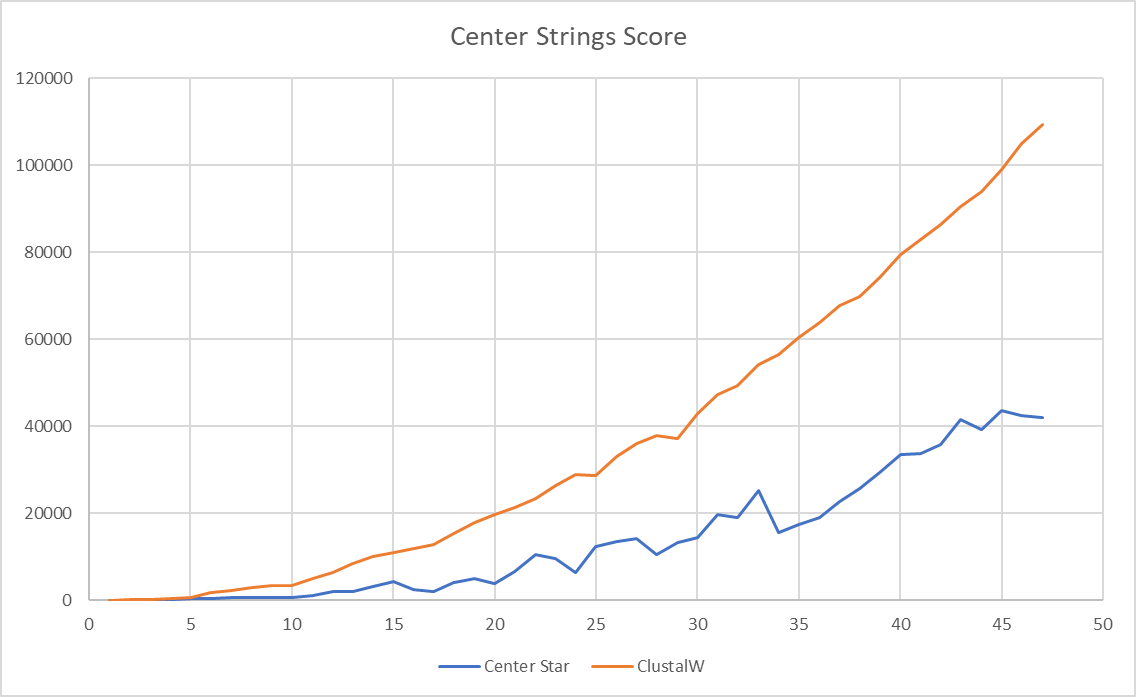
\includegraphics[width=\textwidth]{image001.png}
        \caption{}
        \label{fig:centerScore}
    \end{subfigure}
    ~
    \begin{subfigure}[b]{0.49 \textwidth}
        \centering
        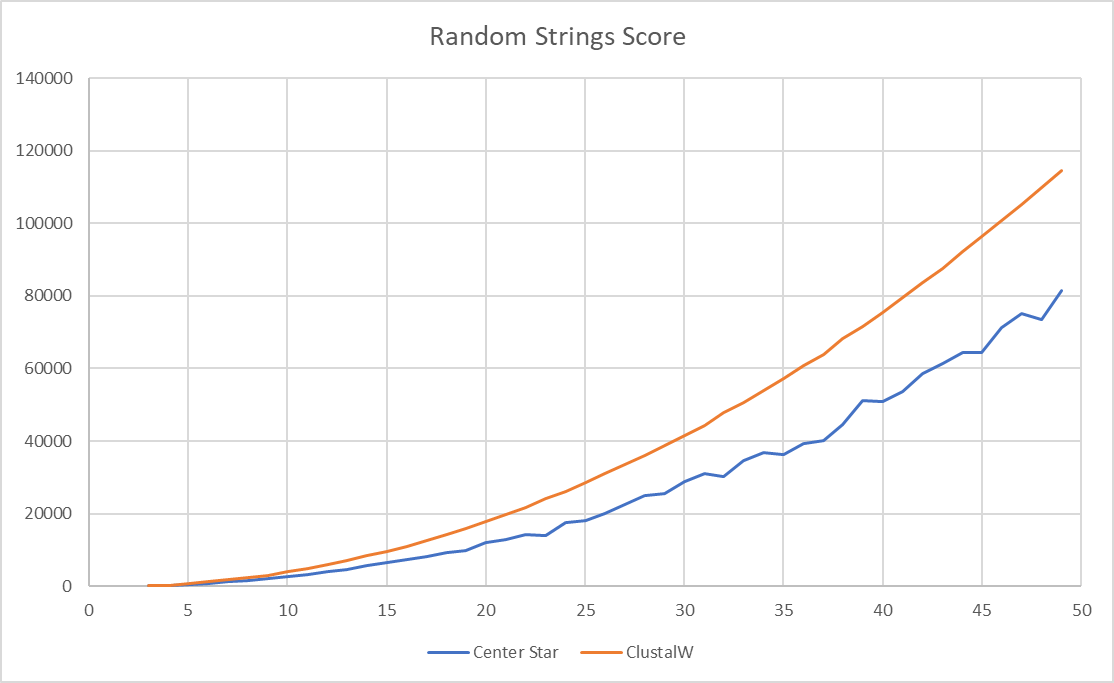
\includegraphics[width=\textwidth]{image003.png}
        \caption{}
        \label{fig:randomScore}
    \end{subfigure}
    ~
    \begin{subfigure}[b]{0.49 \textwidth}
        \centering
        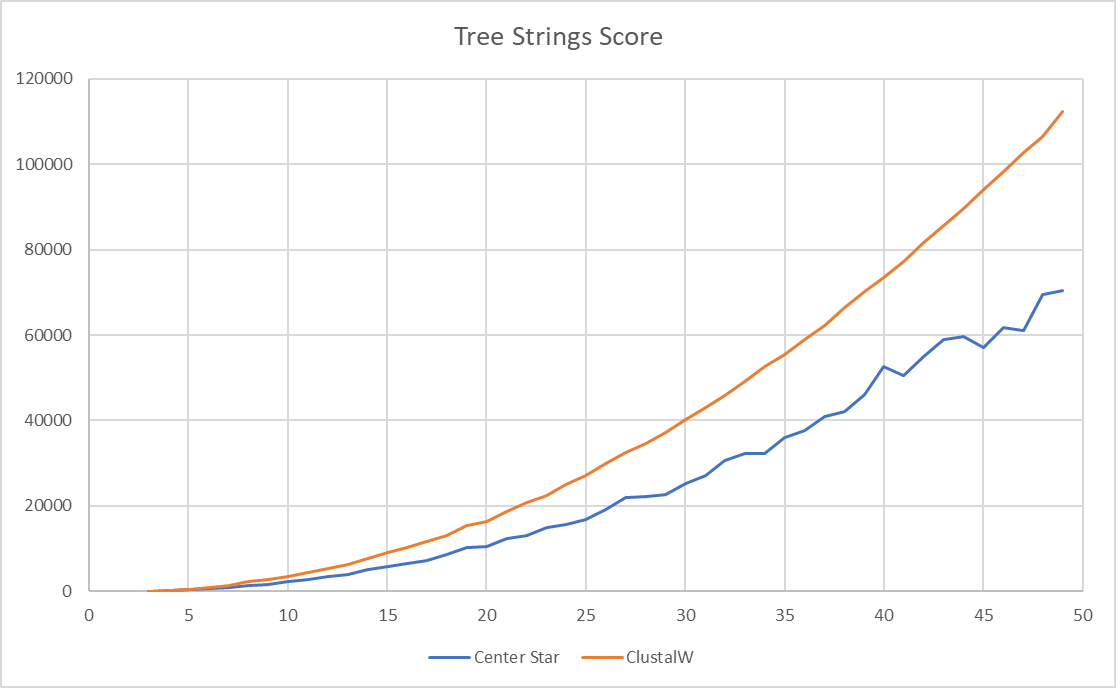
\includegraphics[width=\textwidth]{image013.png}
        \caption{}
        \label{fig:treeScore}
    \end{subfigure}
    ~
    \begin{subfigure}[b]{0.49 \textwidth}
        \centering
        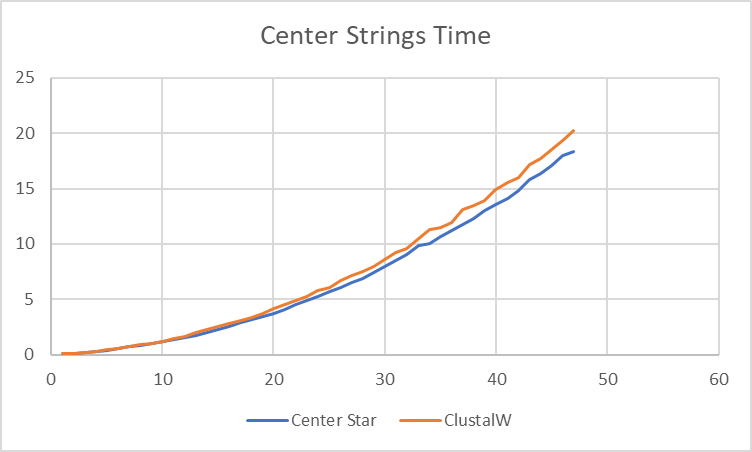
\includegraphics[width=\textwidth]{image002.png}
        \caption{}
        \label{fig:centerTime}
    \end{subfigure}
    ~
    \begin{subfigure}[b]{0.49 \textwidth}
        \centering
        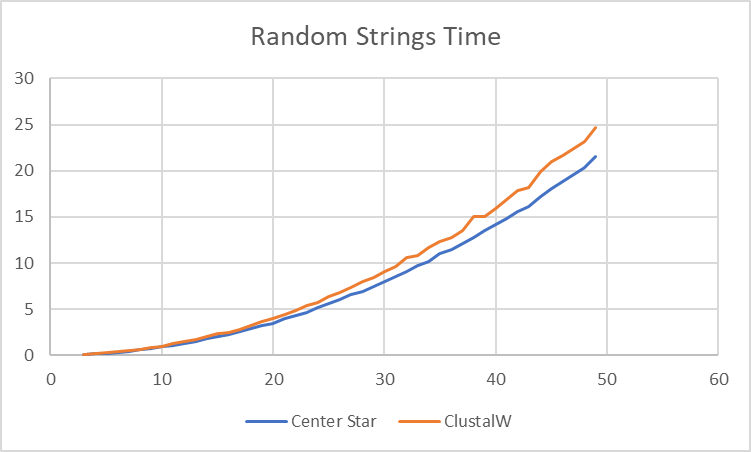
\includegraphics[width=\textwidth]{image004.png}
        \caption{}
        \label{fig:randomTime}
    \end{subfigure}
    ~
    \begin{subfigure}[b]{0.49 \textwidth}
        \centering
        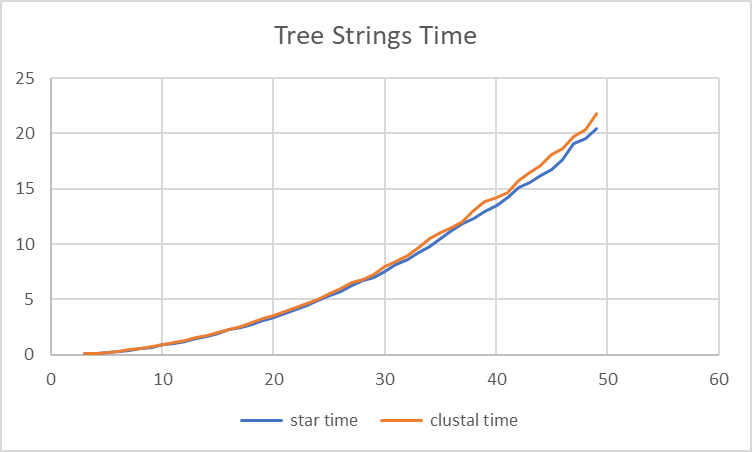
\includegraphics[width=\textwidth]{image009.png}
        \caption{}
        \label{fig:treeTime}
    \end{subfigure}
    \caption{Results showing running time and MSA scores on different string generation strategies}
    \label{fig:all_results}
\end{figure}

\section{Discussion}
The results were quite surprising.
I expected ClustalW to perform significantly better than CenterStar.
However it clearly did not. 
I have no idea why.
It is possible that my data was too synthetic
and the algorithm got no benefit from using the guide tree.

The running time makes sense. Both are fairly similar, but ClustalW has an extra $k^3$ term
so it makes sense that it would be slower.
Both of the running times are so much shorter than the exact algorithm.
It is absolutely absurd! I did not expect the optimal algorithm to be so slow.
It takes over 15 minutes to solve only four strings of length 50!
This is quite small in the grand scheme of things. 
I hadn't anticipated the exponential term being so brutal at increasing real running time.

In terms of implementation details, ClustalW was very hard.
It requires 2 very non-trivial algorithms in order to work.
There is also a non-zero chance that the performance of ClustalW is simply due to implementation error.
I do not see where I went wrong, but I had to make several assumptions about what lines of code meant.


\nocite{*}
\singlespacing
\bibliographystyle{plain}
\bibliography{refs}



\end{document}